\documentclass[12pt]{article}
\usepackage[utf8]{inputenc}
\usepackage[spanish]{babel}
\usepackage{listings}
\usepackage{graphicx}
\graphicspath{ {images/} }
\usepackage{cite}


\begin{document}
\large
\begin{titlepage}
    \begin{center}
        \vspace*{1cm}
            
        \Huge
        
        \textbf{Taller Memoria}
            
        \vspace{0.5cm}
        \LARGE
    
            
        \vspace{3cm}
            
        \textbf{Javier José León Rodriguez}
            
        \vfill
            
        \vspace{0.8cm}
            
        \Large
        Despartamento de Ingeniería Electrónica y Telecomunicaciones\\
        Universidad de Antioquia\\
        Medellín\\
        Septiembre de 2020
            
    \end{center}
\end{titlepage}

\tableofcontents
\vspace{0.5cm}
\section{La memoria del computador.}
La memoria del computador hace referencia al dispositivo encargado del almacenamiento temporal de informacion que está activa en el momento, esto quiere decir que una vez se ha acabado de trabajar con dicha información la memoria procedera con nueva informacion activa del momento. Es preciso resaltar que la terminologia correcta para este componente se denomida Memoria de acceso aleatorio o tambien conocida por sus siglas como RAM.

 \vspace{0.5cm}
 

\section{Tipos de memoria.} \label{contenido}
En tanto a lo que el almacenaje de la computadora se refiere, se han ido desarrollando distintos tipos de memoria con crecientes niveles de optimización y con propósitos específicos que desempeñan importantes labores a la hora de almacenar, organizar y priorizar la información; si bien algunas pueden cumplir labores parecidos, es muy importante dar a conocer cual es la función específica de cada una de estas dentro del sistema de almacenaje computacional.Por tanto, en orden jerarquico de más veloz a menos veloz, las memorias son las siguientes:
\begin{itemize}
\vspace{15PT}
\textbf{Memoria caché :}

Esta es la memoria encargada de almacenar la información que es más habitualmente utilizada. los procesos que requieren mayor trabajo y desempeño son asignados a la memoria caché puesto que esta es la más eficiente a la hora de trabajar con la información, cabe aclarar que la recopilación de dicha información es sacada directamente desde la memoria RAM, sin embargo, la memoria caché se encuentra compuesta por niveles en donde similarmente a la relación entre la memoria RAM y la memoria caché, la información es nuevamente priorizada debido a que la memoria caché está compuesta de ciertos niveles en donde la información que se prioriza es la cual  trabaja a la par del procesador y que será asignada al primer nivel(L1) de la memoria, puesto que es información rápida y ligera, así mismo la información que es menos utilizada se le es asignada al nivel 2(L2) de la memoria caché, y de esta misma manera al último nivel denominado nivel 3 (L3).
\newline
\begin{figure}[h]
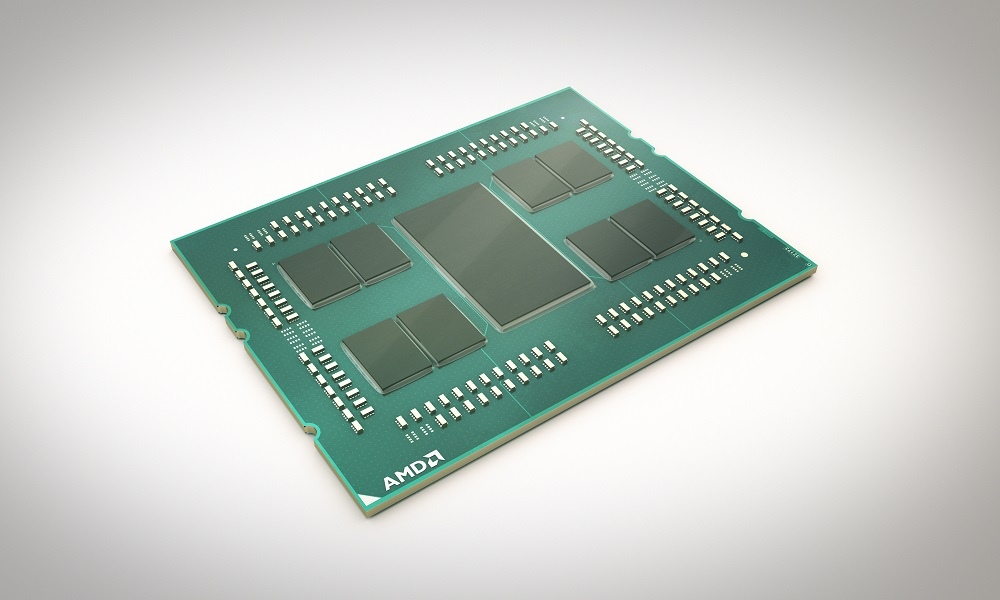
\includegraphics[width=4cm]{caché.jpg}
\centering
\caption{Memoria caché}
\label{fig:RAM}
\end{figure}
\vspace{15PT}
\newline
\textbf{Memoria RAM}: La memoria RAM (el significado de sus siglas es Memoria de Almacenamiento Aleatorio), esto quiere decir que la información almacenada en esta es muy fácil de administrar, en donde, la información que se precisa es asignada una celda para cada bit de información, a diferencia de la memoria de acceso serial (SAM) en donde la información se encuentra en un solo punto especifico de la misma, por lo tanto una vez se recorra la información contenida en esta, se deberá de pasar por cada uno de los puntos anteriores a la información que se desea obtener, ralentizando notablemente e proceso de manejo de la información, sin ella la computadora se vería imposibilitada para funcionar correctamente. Esta memoria es considerada como la más importante dentro del conjunto de memorias; se emplea para almacenar temporalmente las instrucciones o los datos. Este tipo de memoria informática también se le conoce como memoria de escritura y lectura, porque pueden leerse o escribirse los datos en ella, este proceso es realizado mediante copias de información inicial suministrada por el disco duro, debido a esto, popularmente se dice que la memoria RAM solo trabaja mientras la computadora se encuentra encendida, una vez la computadora es apagada la información contenida en la RAM procede a desecharse. Esta memoria se encarga principalmente desde algunos procesos temporales, tales como las modificaciones en los archivos, hasta todas aquellas instrucciones que hacen posible que se ejecuten las aplicaciones que tenemos instaladas en nuestro ordenador.

\newline

\textit{Referencias acerca Memoria RAM}
\cite{conociendo}
\cite{dos}

\begin{figure}[h]
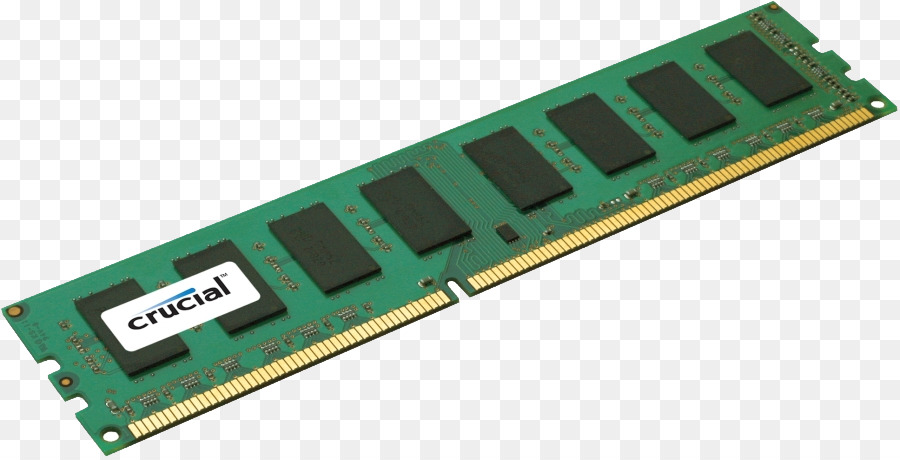
\includegraphics[width=4cm]{RAM1.jpg}
\centering
\caption{Memoria RAM}
\label{fig:RAM}
\end{figure}

\newline

\vspace{15PT}
\newline
\textbf{Memoria virtual}:Esta memoria es basada directamente a la relación entre el disco duro y la memoria RAM en tanto a que la información que maneja en esta no es prioritaria, por lo tanto una fracción del disco duro se encarga de administrar dicha información de baja relevancia,por lo tanto es seguro asegurar que la información almacenada en  esta memoria se maneja de forma más lenta en comparación a la memoria RAM, sin embargo, esta información no es desechada, en su lugar esta es dejada a una lado en espera a ser reactivada cuando esta sea precisa, de este modo podemos decir que la memoria virtual se encarga principalmente de las tareas que se dejan en segundo plano mientras que la memoria RAM es la que lleva a cabo información de primer plano.
\vspace{15PT}
\newline
\textbf{Disco duro:} Es el encargado de almacenar datos a largo plazo, los cuales no se eliminan al apagar la computadora, sin embargo, este presenta un gran problema en cuanto al manejo de la información se refiere, esto debido a su arquitectura que complica la navegación por su información al ser muy lenta en comparación a los anteriores dispositivos de memoria mencionados. Aún con su gran desventaja es necesario conocer el hecho de que, el disco duro es netamente el dispositivo sobre el cual los demás periféricos y dispositivos trabajan, esto contribuye a idea de que la verdadera información real solo existe en el disco duro tanto en el momento en que la computadora está encendida como apagada; lo anterior es correcto asumiendo que la información que se maneja en las diferentes memorias mencionadas anteriormente tan solo con copias de la información original sobre las que se trabaja y esta solo existe mientras el computador está llevando a cabo tareas o procedimientos.
\begin{lstlisting}
\end{lstlisting}
\end{intermize}


\section{Como se gestiona la memoria en un computador}
Esta se gestiona clasificando, priorizando y filtrando la información que cada memoria (incluyendo sus componentes) debe de manejar, es decir, existe información específica que cada memoria debe de manipular, eso se hace con el motivo de facilitar las tareas que cada memoria manipula, liberando en gran medida la carga que cada una de las memorias tiene que manejar y por lo tanto se consigue más desempeño en sus funciones. Cabe aclarar que la clasificación de la información que estas memorias manejan son consecuencia en gran parte al almacenamiento que estas poseen, por lo tanto existe una relación en donde, la información que es manejada por las memorias que poseen un bajo almacenamiento, compensan su desventaja con un alto desempeño de sus funciones.
\label{conclulsion}

\bibliographystyle{IEEEtran}
\section{¿Qué hace que una memoria sea más rápida que otra?, ¿Por qué esto es importante?}
Varios factores juegan un papel importante en cuanto al desempeño de las memorias se refiere, como pueden ser, la arquitectura que las compone, la capacidad de almacenaje de estas y el tipo de información con el que trabajan, un ejemplo claro de esto es que podemos darnos cuenta a medida que avanzamos en la jerarquía de memorias, a medida que el almacenamiento de estas aumenta, tanto su desempeño como velocidad se ve reducido. No obstante, lo que realmente define que una memoria sea más veloz que otra es en gran parte al último aspecto mencionado, es decir, el tipo de información con el que cada una de estas trabaja, manipula y prioriza, Aunque a simple vista este sistema pareciera dar problemas debido a que la capacidad que cada memoria varía en gran cantidad entre ellas, la ingeniería computacional se las ha apañado para optimizar el trabajo que la computadora debe realizar para con el manejo de la información, esto es posible por medio de la clasificación de la información que cada memoria debe de manipular, por ejemplo, una característica clara que notamos al momento de descender en la jerarquía de las memorias es, la memoria que se encuentra en el tope jerárquico es la que maneja la información previamente filtrada por las que la suceden, por tanto, esta información al momento de ser recibida por la memoria anteriormente mencionada, llega con cierto grado de filtración y por ende, es información que ha sido priorizada para ser manipulada por pequeñas cantidades de almacenaje, esta astuta idea nace debido a que la experiencia del usuario requiere de respuestas inmediatas de la computadora como pueden ser las tareas ejecutadas en primer plano o la información que más repetidamente se utiliza, dichas tareas son llevadas a cabo por las memorias más veloces del conjunto de memorias, por lo que en cierto modo, se crea una ilusión de rapidez computacional, en donde la información que se ejecuta en segundo plano si bien no está siendo trabajada, puede ser potencialmente utilizada por el usuario, seguido a esto tenemos información de más baja prioridad que si bien se está ejecutando en segundo plano, es información que ejecuta a otra de mucha más prioridad, como lo es el sistema operativo.
\newline
\newline
\textit{Gran parte de este documento es referenciado gracias al domuneto del Docente.}
\newline
\cite{Doc}
\label{conclulsion}
\bibliographystyle{Outran}
\bibliography{references}
\end{document}
